\documentclass{sep}
\usepackage{lipsum} % For placeholder text
\usepackage{graphicx}
\usepackage{subcaption}
\usepackage{hyperref}
\usepackage{xcolor}
\usepackage{graphicx}
\usepackage{times}
\usepackage{newtxtext}
\usepackage{letterspace}
\usepackage{amssymb}
\usepackage{rotating,tabularx}
\usepackage{amsmath}
\usepackage{graphicx}
\usepackage{tocloft}
\usepackage{indentfirst}
\usepackage{makeidx}
\usepackage{booktabs}
\usepackage{multicol}
\usepackage{multirow}
\usepackage{polski}
\usepackage{gensymb}
\usepackage{listings}
\usepackage{float}
\usepackage{lscape}
\usepackage{bold-extra}
\usepackage{hyperref}	
\usepackage{caption}
\usepackage{xurl}




\addbibresource{references.bib}

\title{Tytuł pracy dyplomowej}
\author{mgr inż. Imię Nazwisko Autora}
\degreefield{kierunek studiów}
\fieldofstudy{kierunek studiów}
\supervisor{prof. dr hab. inż. Imię Nazwisko Promotora}
\department{Katedra w Której Zatrudniony Jest Promotor}

\begin{document}

\maketitle

\textbf{Abstract.}
Tekst streszczenia pracy dyplomowej należy napisać czcionką Times New Roman o rozmiarze 10 pkt z wyrównaniem dwustronnym. Między wierszami streszczenia należy stosować odstęp pojedynczy. Całość przygotowanego streszczenia winna zająć kilka stron formatu B5 (176x250 mm) (minimum 4). Marginesy: lewy prawy górny 2 cm dolny 23 cm. Zastosować formatowanie nagłówka stopki tytułu pracy oraz imiona i nazwiska autorów zgodnie z niniejszym wzorcem.

W abstrakcie umieścić zwięzły opis treści streszczenia pracy dyplomowej wraz z wnioskami końcowymi. Kilka zdań opisujących podjęte w pracy dyplomowej działania. Pokrótce opisana problematyka użyte narzędzia lub zastosowane podejście a także uzyskane efekty. Abstrakt powinien zostać napisany językiem "pop-science" aby był zrozumiały dla każdego odbiorcy "laika" zachęcając do lektury całego artykułu. W streszczeniu proszę nie cytować literatury. Objętość abstraktu nie powinna przekraczać 15 wierszy (100-150 wyrazów).
\section{Cel i założenia}
Pierwszy rozdział streszczenia powinien zawierać ogólne informacje na temat pracy dyplomowej. Zazwyczaj zawiera informacje zawarte w Karcie pracy dyplomowej. Dwa-trzy zdania dotyczące celu realizowanej pracy oraz założenia projektowe. Założenia projektowe należy sformułować w postaci punktów (prawdopodobnie tak jest w Karcie pracy dyplomowej). Przed założeniami musi znaleźć się zdanie które stanowi wprowadzenie do założeń np.: Główne założenia projektowe realizowanej pracy to:
\begin{itemize}
	\item elementy listy punktowanej rozpoczynamy małą literą,
	\item i kończymy przecinkiem,
	\item wyjątkiem jest ostatni punkt który zaczynamy małą literą ale kończymy kropką.
\end{itemize}

\section{Wstęp teoretyczny}
W tym rozdziale proszę opisać wszystkie najważniejsze do zrozumienia dalszej części treści teoretyczne. Wszystkie powszechnie znane fakty muszą być odpowiednio zacytowane. Do tego zadania wykorzystuje się odpowiednie polecenie LaTeXa, proszę nie wpisywać literatury "ręcznie" w nawiasach \cite{poz1}. Jeśli fragment napisany jest na podstawie więcej niż jednego źródła, proszę w nawiasie wymienić wszystkie pozycje literaturowe, oddzielając je przecinkiem \cite{poz1, poz2, poz3, poz4}. Polecenie \textit{cite} wykona odpowiednie formatowanie, skracając cytowanie tak, jak jest poprawnie \cite{poz5, poz6}. Wzory pojawiające się w treści wprowadza się wraz z ich numeracją. Każdy z wzorów musi mieć odwołanie w tekście. Proszę unikać zdań "poniższy wzór opisuje", na rzecz: "na równaniu \eqref{eq:nazwisko_1} przedstawiono równanie opisujące zależność wiążącą pięć najważniejszych liczb matematyki".
\begin{equation}
	e^{\pi i }-1 = 0
	\label{eq:nazwisko_1}
\end{equation}
Odwoływania się do konkretnego numeru równania dokonuje się za pomocą polecenia \textit{eqref}, dzięki czemu numer umieszczony jest w nawiasie okrągłym. Odwołania do pojawiających się rysunków lub tabel wykonujemy za pomocą polecenia \textit{ref}. W tekście liczby od jednostek muszą być rozdzielone spacją i pisane tekstem prostym - przykład: $230 \textrm{V}$.
\section{Projekt i wykonanie}
W tym rozdziale powinien znaleźć się opis działań podjętych w realizacji pracy dyplomowej. W poniższych punktach szablonu zostanie przedstawione przykładowe formatowanie mogących pojawić się elementów. Należy mieć na uwadze, że niedopuszczalne jest umieszczanie podpunktów bezpośrednio pod punktami/sekcjami. Każdy duży punkt (sekcja) musi zawierać przynajmniej jedno zdanie, zanim wprowadzony zostanie podrozdział/tabela lub obrazek.
\subsection{Podrozdział 1}
W przypadku podrozdziału obowiązuje zasada taka jak w przypadku rozdziału - na początku musi pojawić się zdanie tekstu, podrozdział nie może rozpoczynać się tabelą lub rysunkiem. Wprowadzony podrozdział, nie może być jedynym podrozdziałem w danym rozdziale. Inaczej zastosowanie podrozdziału jest nieuzasadnione. 
\subsection{Rysunki}
Wprowadzanie do treści rysunków może odbywać się na kilka sposobów. W każdym jednak przypadku musi wystąpić odwołanie do rysunku w treści streszczenia. Wszystkie obrazki proszę umieścić w folderze "rysunki" w możliwie najwyższej jakości. W miarę możliwości proszę nazwać je kolejnymi liczbami naturalnymi, w kolejności występowania w tekście. Rysunek \ref{fig:nazwisko_1} przedstawia podstawowy sposób osadzania rysunków w treści.
\begin{figure}[H]
	\centering
	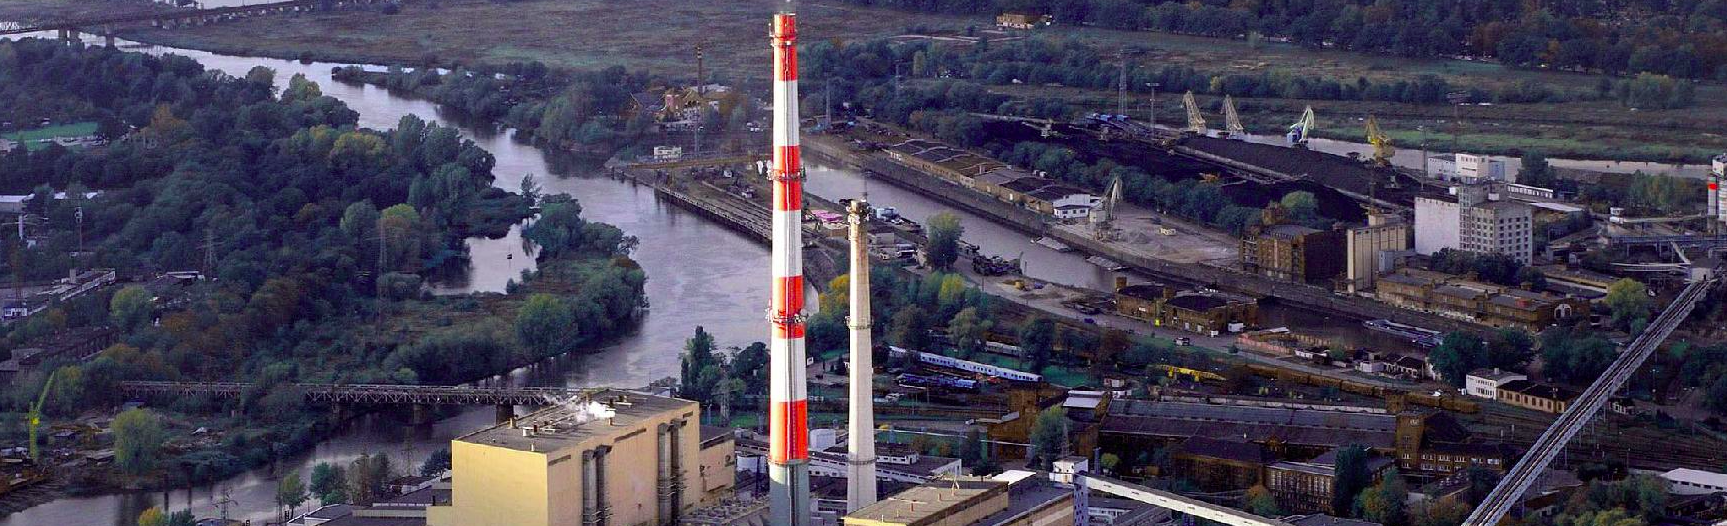
\includegraphics[width=\linewidth]{figures/1.png}
	\caption{Przykład osadzenia rysunku w treści - tytuł zakończony kropką. \label{fig:nazwisko_1}}
\end{figure}
%Użycie opcji pozycjonowania obrazu [H] umieści obrazek dokładnie w tym miejscu, w którym Państwo chcą - gdy nie zmieści się na stronie, zostanie przeniesiony na nową stronę, pozostawiając puste miejsce na poprzedniej. Przykład umieszczenia kilku obrazków obok siebie z jednym podpisem przedstawia rysunek \ref{fig:nazwisko_2}. W zależności od wyboru wymiarów (szerokości lub wysokości) obrazka, będą one rozmieszczone w jednym lub więcej rzędów. Odwołanie do konkretnego obrazka na rysunku analogicznie jak do całego rysunku (rysunek \ref{fig:nazwisko_2}\subref{fig:nazwisko_2_2}).
\begin{figure}[H]
	\centering
	\subfloat[podpis 1]{
\includegraphics[width=.3\linewidth]{figures/2.png}\label{fig:nazwisko_2_1}} 
	\hspace{.4em} %szerokość odstępu można ewentualnie zmniejszyć, w razie potrzeby
	\subfloat[podpis 2]{
\includegraphics[width=.3\linewidth]{figures/2.png}\label{fig:nazwisko_2_2}} 
	\hspace{.4em}
	\subfloat[podpis 3]{
\includegraphics[width=.3\linewidth]{figures/2.png}\label{fig:nazwisko_2_3}}
	\caption{Podpis dotyczący wszystkich obrazków. \label{fig:nazwisko_2}}
\end{figure}
W sytuacji, gdy podpis do każdego z obrazków wchodzących w skład rysunku jest długi, można obrazki podpisać jedynie literami, a treść umieścić w podpisie do całego rysunku. Przykład przedstawia rysunek \ref{fig:nazwisko_3}.
\begin{figure}[H]
	\centering
	\subfloat[]{
\includegraphics[width=.3\linewidth]{figures/2.png}\label{fig:nazwisko_3_1}} 
	\hspace{.4em} %szerokość odstępu można ewentualnie zmniejszyć, w razie potrzeby
	\subfloat[]{
\includegraphics[width=.3\linewidth]{figures/2.png}\label{fig:nazwisko_3_2}} 
	\caption{Podpis dotyczący wszystkich obrazków, \protect\subref{fig:nazwisko_3_1} - podpis 1, \protect\subref{fig:nazwisko_3_2} - podpis 2.}
	\label{fig:nazwisko_3}
\end{figure}
\subsection{Tabele}
Do wszystkich pojawiających się w treści tabel, podobnie jak do rysunków, musi prowadzić odwołanie w tekście. Każda tabela, podobnie jak rysunek, musi mieć tytuł - w przypadku tabeli umieszczony nad nią. W miarę możliwości należy unikać pionowych linii w tabelach. Należy również używać odpowiednich komend do rysowania linii nad i pod tabelą, oraz linii środkowych. Tabela \ref{tab:nazwisko_1} przedstawia przykład formatowania. W miarę możliwości pojawiające się liczby rozdzielamy separatorem tysięcznym w postaci białego znaku - spacji, zaś części dziesiętne rozdzielać przecinkami, przykład: 1 230,76.

\begin{table}[H] 
	\renewcommand{\arraystretch}{1.3}
	\footnotesize
	\caption{Tytuł tabeli zakończony kropką. \label{tab:nazwisko_1}}
	\newcolumntype{C}{>{\centering\arraybackslash}X}
	\begin{tabularx}{\textwidth}{CCC}
		\toprule
		\textbf{Tytuł 1}	& \textbf{Tytuł 2}	& \textbf{Tytuł 3}\\
		$[\textrm{Hz}]$ & $\cdot 10^{-6}[\textrm{s}]$ & $[\frac{\textrm{m}}{\textrm{s}}]$\\
		\midrule
		Nagłówek 1		& Data			& Data\\
		Nagłówek 2		& Data			& Data\\
		Nagłówek 3		& Data			& Data\\
		Nagłówek 4		& Data			& Data\\
		\bottomrule
	\end{tabularx}
\end{table}

W przypadku, gdy w tabeli zawarte są wielkości fizyczne, niezbędne jest określenie ich wymiaru - w miarę możliwości należy podać je w pierwszym wierszu, w kwadratowych nawiasach, prostym tekstem. Przykład zawiera tabela \ref{tab:nazwisko_1} - należy używać polecenie \textit{textrm}.

W przypadku, gdy tabela, którą chcą Państwo przedstawić jest zbyt szeroka, by umieścić ją na stronie można użyć strony poziomej. Przykład tabeli umieszczonej na poziomej stronie - tabela \ref{tab:nazwisko_2}. W przypadku umieszczenia poziomej strony niezbędne jest użycie komendy \textit{newpage} po tabeli, wymuszającej wykonane nowej strony. 
\begin{sidewaystable}[ph!]
	\renewcommand{\arraystretch}{1.3}
	\footnotesize
	\caption{Tytuł poziomej tabeli zakończony kropką. \label{tab:nazwisko_2}}
	\newcolumntype{C}{>{\centering\arraybackslash}X}
	\begin{tabularx}{\textwidth}{CCCCC}
		\toprule
		\textbf{Tytuł 1}	& \textbf{Tytuł 2}	& \textbf{Tytuł 3} & \textbf{Tytuł 4}	& \textbf{Tytuł 5}\\
		$[\textrm{Hz}]$ & $\cdot 10^{-6}[\textrm{s}]$ & $[\frac{\textrm{m}}{\textrm{s}}]$ & $[\textrm{m}]$ & $[\mu\textrm{m}]$\\
		\midrule
		Nagłówek 1		& Data			& Data      & Data			& Data\\
		Nagłówek 2		& Data			& Data      & Data			& Data\\
		Nagłówek 3		& Data			& Data      & Data			& Data\\
		Nagłówek 4		& Data			& Data      & Data			& Data\\ \midrule
		Nagłówek 5		& Data			& Data      & Data			& Data\\
		Nagłówek 6		& Data			& Data      & Data			& Data\\
		Nagłówek 7		& Data			& Data      & Data			& Data\\
		Nagłówek 8		& Data			& Data      & Data			& Data\\ \midrule
		Nagłówek 9		& Data			& Data      & Data			& Data\\
		Nagłówek 10		& Data			& Data      & Data			& Data\\
		Nagłówek 11		& Data			& Data      & Data			& Data\\
		Nagłówek 12		& Data			& Data      & Data			& Data\\
		\bottomrule
	\end{tabularx}
\end{sidewaystable}
\newpage
\section{Uzyskane wyniki}
W tym rozdziale proszę omówić uzyskane przez Państwa wyniki. Tabele, wykresy. W miarę możliwości w jak najlepszej jakości. Jeśli wykresy rysowane były w programie Excel (lub istnieją dane źródłowe zawierające dane do wykresów), proszę dołączyć pliki z danymi - to pozwoli uzyskać możliwie najlepszą jakość i ustalić formatowanie takie same dla wszystkich rozdziałów w monografii. Rozdział ten można również podzielić na podrozdziały, zasady obowiązują bez zmian (przynajmniej jedno zdanie przed wprowadzeniem podrozdziałów, przynajmniej dwa podrozdziały).
\section{Podsumowanie}
Podsumowanie musi zawierać najważniejsze wnioski wynikające z przeprowadzonych i przedstawionych badań. Proszę pamiętać, by podsumowania nie formułować w postaci punktów, a w postaci zdań. Podsumowanie powinno stanowić około 10\% objętości artykułu. Zatem, dla artykułu o 5-10 stronach powinni Państwo sformułować 0.5-1.0 stronę podsumowania. Gdy w podsumowaniu odwołują się Państwo do danych pochodzących z innych źródeł niż streszczana praca (np. gdy porównują Państwo uzyskane wyniki z wynikami innych naukowców), proszę nie zapomnieć o odpowiednim cytowaniu \cite{poz3}. W przypadku, gdy chcą Państwo opisywać wyniki przedstawione na rysunku lub tabeli, proszę odpowiednio się do nich odwołać (rysunek \ref{fig:nazwisko_1}, tabela \ref{tab:nazwisko_2}), by Czytelnik nie miał wątpliwości o czym dokładnie Państwo piszą.

Proszę pisać treść, posługując się poprawną polszczyzną - zarówno w kontekście ortografii, jak i interpunkcji.
Proszę przesłać plik w wersji edytowalnej (.tex).

Bibliografię proszę posortować według kolejności występowania w tekście. Wszystkie pozycje w bibliografii muszą mieć odniesienie w tekście. W przypadku cytowania:
\begin{itemize}
	\item \textsc{artykułu} - najpierw autorzy w formacie: Nazwisko I., następnie tytuł cytowanego artykułu, tekstem zwykłym. Kolejno nazwa czasopisma czcionką pochyłą, dalej rok wydania - pogrubiony, kolejno numer tomu, a na końcu strony, na których umieszczony został artykuł. Poszczególne elementy rozdzielić przecinkami, pozycję zakończyć kropką.
	\item \textsc{książki} - najpierw autorzy w formacie: Nazwisko I. tekstem zwykłym, następnie tytuł cytowanej książki pisany kursywą, następnie numer wydania, nazwa wydawnictwa, miejsce i kraj siedziby wydawnictwa, rok wydania książki. Poszczególne elementy rozdzielić przecinkami, pozycję zakończyć kropką.
	\item \textsc{rozdziału w książce} - najpierw autorzy w formacie: Nazwisko I., następnie tytuł cytowanej części książki (np. rozdziału) pisane tekstem zwykłym, następnie W: nazwa książki pisany kursywą, kolejno nazwisko edytora, nazwa wydawnictwa, miejsce i kraj siedziby wydawnictwa, rok wydania książki, zakres stron, na których umieszczony jest cytowany fragment. Poszczególne elementy rozdzielić przecinkami, pozycję zakończyć kropką.
	\item \textsc{referatu konferencyjnego} - najpierw autorzy w formacie: Nazwisko I., następnie tytuł treści konferencyjnej (prezentacji/artykułu) pisane tekstem zwykłym, następnie nazwa konferencji, miejsce odbywania konferencji (miasto, kraj), data konferencji (Dzień Miesiąc Rok). Jeśli opublikowano fragment w materiałach konferencyjnych, można umieścić numer abstractu oraz zakres stron. Poszczególne elementy rozdzielić przecinkami, pozycję zakończyć kropką.
	\item \textsc{strony internetowej} - najpierw tytuł strony, następnie zdanie "Dostępny online:" oraz adres strony internetowej, kolejno w nawiasie okrągłym: "dostęp" i data uzyskania dostępu w formacie DD-MM-YYYY. Pozycję zakończyć kropką.
	\item \textsc{pracy dyplomowej} - najpierw autor w formacie: Nazwisko I. tekstem zwykłym, następnie tytuł pracy dyplomowej, kolejno poziom (praca inżynierska, praca magisterska, rozprawa doktorska), nazwa uczelni nadającej tytuł, miasto i kraj lokalizacji uczelni oraz data złożenia pracy w formacie DD-MM-YYYY. Poszczególne elementy rozdzielić przecinkami, pozycję zakończyć kropką.
\end{itemize}


\printbibliography

\end{document}
